\documentclass[a4paper,oneside,openany,12pt]{memoir}
\usepackage[T1]{fontenc} % To get different font encoding, thus allow \guillemotright.
\usepackage{graphicx} % For images
\graphicspath{{../gfx/}}
%\usepackage[english]{babel} % For correct word hyphenating.
\usepackage{color} % For the colored boxes.
\usepackage{hyperref} % For URLs.
\usepackage{float} % For custom floats (the info boxes) and a box around every figure.
% When loaded before float, doesn't work. When loaded after, it's included *within* the fbox.
% Maybe not do an fbox but a box without border and with background color?
%\usepackage[format=hang,font=footnotesize,labelfont=bf]{caption} % To format captions.

% Include all of this in a separate file!
\newcommand{\HRule}{\rule{\linewidth}{1mm}} % Doet height (zie style) hetzelfde?
\newcommand{\institute}[1]{\gdef\inst{#1}}  % Beamer supplies \institute. We want that, too.
\newcommand{\inst}{}                        % Beamer supplies \institute. We want that, too.
\newcommand{\funding}[1]{\gdef\fund{#1}}    % Provide funding line.
\newcommand{\fund}{}                        % Provide funding line.
\newcommand{\setLOVDversion}[1]{\gdef\LOVDversion{#1}} % Provide the current LOVD version.
\newcommand{\LOVDversion}{}                            % Provide the current LOVD version.

\setlrmarginsandblock{2cm}{2cm}{*} % LEFT-RIGHT
\setulmarginsandblock{2cm}{2cm}{*} % TOP-BOTTOM
\checkandfixthelayout % Without this, nothing works. Took me ages before I found out.
\fixpdflayout % Not sure if we need this, but it was recommended someplace.



\makepagestyle{LOVD}

% Because we don't have odd or even pages, we only need to define odd pages.
\makeoddhead{LOVD}{\normalfont\leftmark}{}{\normalfont\rightmark}
\makeheadrule{LOVD}{\textwidth}{\normalrulethickness}
\makeoddfoot{LOVD}{}{\normalfont\thepage}{}
\makefootrule{LOVD}{\textwidth}{\normalrulethickness}{\footruleskip}

% Style "plain" is called from chapters. We want chapters to have a footer as well.
\makeoddfoot{plain}{}{\normalfont\thepage}{}
\makefootrule{plain}{\textwidth}{\normalrulethickness}{\footruleskip}

% Additional changes:
\makepsmarks{LOVD}{%
  \nouppercaseheads

  \createmark{chapter}{left}{shownumber}{}{.\space} % (\leftmark) number, followed by a . and a space.
  \createmark{section}{right}{nonumber}{}{.\space} % (\rightmark) no number, (useless: followed by a . and a space).
  % Change "shownumber" to "nonumber" if you don't want the chapter/section number displayed at the header.

%  \createplainmark{toc}{both}{\contentsname}
%  \createplainmark{lof}{both}{\listfigurename}
%  \createplainmark{lot}{both}{\listtablename}
%  \createplainmark{bib}{both}{\bibname}
%  \createplainmark{index}{both}{\indexname}
%  \createplainmark{glossary}{both}{\glossaryname}
  % Might want to keep those, see the manual for further information.
}
% Activate your new pagestyle
\pagestyle{LOVD}



%\newcommand{\maketitle}{%
%  \vspace*{\droptitle}
%  \maketitlehooka
%  {\pretitle \title \posttitle}
%  \maketitlehookb
%  {\preauthor \author \postauthor}
%  \maketitlehookc
%  {\predate \date \postdate}
%  \maketitlehookd
%  \thispagestyle{title}
%}

\setlength{\droptitle}{-3cm} % Moves the title (logo, title, authors etc) 3cm up.
\pretitle{
  \begin{center}
    
\includegraphics[width=17cm]{logo.jpg}
    \vskip 4cm
    \HRule\par\HUGE\bfseries\sffamily} %% Need proper font!
\posttitle{\par\HRule\end{center}\vskip 3cm}
\preauthor{\flushright}
\postauthor{\par\inst\par\vskip 1cm}
\predate{\hfill Last updated } % \hfill aligns the rest of the line to the right. \flushright would have done the same.
\postdate{\par\vskip 2cm \noindent \small \fund}

\makechapterstyle{LOVD}{%
  \setlength\beforechapskip{10pt} % A small distance just above the new Chapter title.
  \setlength\afterchapskip{20pt} % A small distance between the Chapter title and the text.
  \renewcommand{\chapterheadstart}{\vspace*{\beforechapskip}\hrule height 2pt \medskip} % Nice ruler above the Capter title.
  \renewcommand{\chapnamefont}{\normalfont\large\scshape} % CHAPTER
  \renewcommand{\chapnumfont}{\normalfont\LARGE\scshape} % 1
  \renewcommand{\chaptitlefont}{\normalfont\huge\bfseries\scshape} % e.g. "Introduction"
  \renewcommand{\printchaptername}{} % Empty text instead of "Chapter".
                  \renewcommand{\chapternamenum}{ } % Weet niet wat dit anders doet.
                  \renewcommand{\printchapternum}{\chapnumfont \thechapter} % Weet niet wat dit anders doet.
  \renewcommand{\afterchapternum}{. } % Just a dot after the Chapter number, no new line.
  \renewcommand{\afterchaptertitle}{\par\nobreak\medskip\hrule\vskip\afterchapskip} % Nice ruler below the Capter title.
}
\chapterstyle{LOVD}

% For the colored boxes.
%\definecolor{gray}{rgb}{0.9,0.9,0.9}
%\definecolor{darkgray}{gray}{0.3}
\definecolor{linkblue}{rgb}{0.1, 0, 1}
\hypersetup{
  colorlinks,
  citecolor=linkblue,
  filecolor=linkblue,
  linkcolor=linkblue,
  urlcolor=linkblue
}

% The custom floats.
\definecolor{infoblue}{RGB}{240, 243, 255} %F0F3FF
%\floatstyle{ruled}
%\newfloat{infobox}{h!}{floats}
%\floatname{infobox}{}

\floatstyle{boxed} 
\restylefloat{figure}



\newsavebox{\infobox}
\newlength{\infoboxlength}
\newlength{\infoboxinnerlength}
\setlength{\infoboxlength}{\textwidth}
\addtolength{\infoboxlength}{-2\fboxsep}
\addtolength{\infoboxlength}{-2\fboxrule}
\addtolength{\infoboxlength}{-1.5cm}
\setlength{\infoboxinnerlength}{\infoboxlength}
\addtolength{\infoboxinnerlength}{-6pt}

\newenvironment{infotable}
  {\begin{lrbox}{\infobox}%
    \begin{minipage}[t]{1.5cm}
	  \centering
	  \vspace{0pt}
      
\includegraphics[width=1cm,height=1cm]{lovd_information.png}
    \end{minipage}
   \begin{minipage}[t]{\infoboxlength}\vspace{5pt}\begin{minipage}{\infoboxinnerlength}}
  {\vspace{10pt}\end{minipage}\end{minipage}\end{lrbox}%
   \begin{center}
   \fcolorbox{black}{infoblue}{\usebox{\infobox}}
   \end{center}}

\newenvironment{warntable}
  {\begin{lrbox}{\infobox}%
    \begin{minipage}[t]{1.5cm}
	  \centering
	  \vspace{0pt}
      
\includegraphics[width=1cm,height=1cm]{lovd_warning.png}
    \end{minipage}
   \begin{minipage}[t]{\infoboxlength}\vspace{5pt}\begin{minipage}{\infoboxinnerlength}}
  {\vspace{10pt}\end{minipage}\end{minipage}\end{lrbox}%
   \begin{center}
   \fcolorbox{black}{infoblue}{\usebox{\infobox}}
   \end{center}}



% Standard sizes for images.
\newlength{\imagewidth}
\setlength{\imagewidth}{\textwidth}
\addtolength{\imagewidth}{-2\fboxsep}
\addtolength{\imagewidth}{-2\fboxrule}





\setLOVDversion{3.0-beta-05}
\title{LOVD 3.0 user manual \\\vskip 1cm Build \LOVDversion}
\author{Ivo F.A.C. Fokkema}
\institute{Leiden University Medical Center}
\date{2012-05-31} % I guess it's easier to use this as a "Last modified" column.
\funding{LOVD has received funding from the European Community's Seventh Framework Programme\\(FP7/2007-2013) under grant agreement no 200754 - the GEN2PHEN project.}





\begin{document}

\begin{titlingpage} % We don't want the front to count as page 1.
\maketitle
\end{titlingpage}





\tableofcontents





\chapter{Introduction}

This is the manual for the Leiden Open (source) Variation Database (LOVD) version 3.0.
LOVD 3.0 is a partial rewrite of LOVD 2.0, which first stable release was completed in 2007.
Also, LOVD 3.0 has a greatly improved database model, and includes lots of new features aimed at making LOVD useful for more research environments.
\par
LOVD is designed to provide a flexible, freely available tool for gene-centered collection and display of DNA variations.
LOVD 3.0 extends this idea to also provide patient-centered data storage and storage of NGS data, even of variants outside of genes.
\\
\par
LOVD was developed approaching the ``LSDB-in-a-Box'' idea for the easy creation and maintenance of a fully web-based gene sequence variation database,
that is platform-independent and uses PHP and MySQL open source software only.
The design of the database follows the recommendations of the \href{http://www.hgvs.org/}{Human Genome Variation Society} (HGVS)
and focuses on the collection and display of DNA sequence variations, but it has fully implemented methods for storing complete clinical data as well.
The open LOVD setup also facilitates functional extensions with scripts written by the community.
\\
\par
The development of (then nameless) LOVD started in late 2002, while it was first officially released in January, 2004.
Before that LOVD was only in use by the \href{http://www.DMD.nl/}{Leiden Muscular Dystrophy pages},
as a not-so-modular system with lots of characteristics specific for that website only.
With the official release of LOVD in 2004 the system had become much more dynamic and customizing LOVD was made easy mostly by editing text-files.
\par
In 2004, LOVD became available under the open source license GPL and with the 1.1.0 release most of the text-files had been replaced by online forms
so customizations can be performed through the web interface.
Early in 2005 the \href{http://www.ncbi.nlm.nih.gov/pubmed/15977173}{first LOVD article} was published,
and in 2005 the development of LOVD was more targeted at improving the ease of use of the system.
\\
\par
In 2006 the development of LOVD 2.0 started after the decision was made to rewrite all of LOVD from scratch
to be able to include a long list of upgrade suggestions that were hard to implement in LOVD 1.1.0.
Aimed at modularity and data redundancy, LOVD 2.0 was meant to be a more flexible and more powerful successor of the popular 1.1.0 version
and soon it received the interest of LOVD users eager to try out the all-new version.
\par
With more features being added and bugs fixed rapidly, LOVD 2.0 reached beta stage in April 2007,
after which more and more users started to upgrade their 1.1.0 databases to 2.0.
Finally, in October 2007 LOVD 2.0 reached the stable stage, after which LOVD 2.0 was continuously improved with monthly releases for two years,
after which the releases became less frequent.
LOVD 2.0 is described in the \href{http://www.ncbi.nlm.nih.gov/pubmed/21520333}{second LOVD paper}.
\\
\par
By 2009 it had became clear that although LOVD 2.0 was a great step forward, there were still key improvements to be made.
Since the complexity of necessary changes had become to great to gradually upgrade LOVD 2.0 systems to include these options,
it was again decided to start from scratch writing LOVD 3.0.
This allowed us to redesign the complete data model in full freedom,
although it should still be possible for existing LOVD 2.0 databases to have all data transferred to LOVD 3.0.
\par
LOVD 3.0 adds even more flexibility, allowing users to focus exclusively on sequence variants,
whilst also allowing an exclusive focus on individuals and clinical data, and anything in between.
It will be possible for different submitters to work together cooperatively on the same data.
Searching through the data is improved extensively,
and webservices of many different sources are used to automatically retrieve gene and transcript information.
Also new in 3.0 is full Next Generation Sequencing (NGS) support,
with the ability to import VCF or SeattleSeq formats.
For VCF file imports, LOVD allows for automatic annotation of the variants.
Both formats support the automatic creation of genes and transcripts in the system,
greatly reducing the amount of work required by curators to get LOVD set up for their research data.
\par
LOVD 3.0 reached beta stage in January 2012. Currently, the latest release is \LOVDversion.
Keep an eye on our \href{http://www.lovd.nl/3.0/news}{news page} for the latest information on LOVD 3.0 development.
\\
\par
Where ever you see ``he'' or ``his'' written in this manual, it should read ``he or she'' and ``his or her'' respectively.

\begin{infotable}
Please note that this manual is work in progress.
Since LOVD 3.0 is still under development and the development is the focus of our efforts, most features in LOVD 3.0 are not yet described in this manual.
Also, features described in this manual may become inaccurate or even incorrect in later versions of LOVD 3.0.
Please bear with us while we finish this manual.
\end{infotable}










\chapter{Installing LOVD}

Installing LOVD is a ``piece of cake''.
%If you just want to try out LOVD to play around with it a bit, we recommend using the (link) LOVD local install CD, which we currently have available for Windows.
%This LOVD local install CD will install LOVD and all necessary software on your computer in just a few minutes with virtually no effort.
%This CD requires roughly 200MB free space on your hard drive.
%For production environments (you intend to publish LOVD on your institution's server) we recommend a manual install, for which you may require help from your system administrator.
However, you might require help from your system administrator, since there are a few dependencies that need to be taken care of first.





\section{Before you install}
LOVD is a web-based software project.
Therefore, installation requires a correctly set-up webserver.
LOVD has been extensively tested with the Apache webserver, but any webserver able to run PHP scripts should suffice.
You'll need PHP 5.1.0 or higher and MySQL 4.1.2 or higher.
LOVD may work with other database platforms, but we are not developing for other database backends.
You are welcome to try other database backends and report the results to us, but we can't provide any support for it.
For more information, see the \href{http://lovd.nl/3.0/faq/software}{FAQ about software needed}.
\par
A suitable server with the necessary software installed is available at virtually all (academic) institutions and countless (commercial) hosting providers.
\\
\par
Before installing LOVD, be sure you have the required credentials for connecting to the MySQL database.
You need a \emph{hostname}, \emph{username}, \emph{password} and a \emph{database name} to be able to install LOVD.
If you are installing LOVD on a remote server, be sure to have the FTP username and password to be able to copy the necessary files to the server.



\subsection{Download \& Extract}
To download LOVD, go to the \href{http://www.LOVD.nl/3.0/}{LOVD website} and click on the `Download' tab.
You can download LOVD in two formats; GZIPped TARball and ZIP archive.
The first format is common for Unix and Linux systems while the ZIP archive is popular on the Windows platform.
Usually you will be able to open both formats.
\\
\par
Download the file of your choice and save it to your hard drive.
Now extract the file using GZIP/TAR or ZIP to the desired location.
On a server, common directories may be /var/www on Unix or Linux servers, or C:\textbackslash{}htdocs on a Windows server.
To be sure, consult the documentation of the webserver software you are using.



\subsection{Pre-install Setup}
You will need to rename the standard config file config.ini.php-lovd to config.ini.php and edit it in, for example, a basic text editor.
This is absolutely mandatory, because you will need to enter the MySQL hostname, database name, username and password here.
\par
Please go through the entire config.ini.php file to determine if you need to change any of the other settings.

\begin{warntable}
A .htaccess file is put in the root directory of your LOVD installation protecting the config.ini.php file.
This will prevent the config file from being accessed by others on Apache HTTP servers (if configured properly), the most commonly used webserver.
If you use Apache, please check that your version and configuration support this feature.
Make sure you have the .htaccess file into your LOVD directory, on Unix and Linux systems it's a hidden file so it can be missed easily.
For the .htaccess file to work, you need to have ``Limit'' and ``Options'' enabled in Apache's ``AllowOverride'' setting.
\par
Also, make sure you have MultiViews or mod\_rewrite enabled. This allows a PHP file like ``/setup.php'' to be accessed as ``/setup''.
\\
\par
\noindent
More information about .htaccess files:\\
\url{http://httpd.apache.org/docs/2.0/howto/htaccess.html}
\\
\par
\noindent
More information about AllowOverride:\\
\url{http://httpd.apache.org/docs/2.0/mod/core.html\#allowoverride}
\\
\par
\textbf{If you use a different webserver}, make sure to configure it to deny access to the config.ini.php file.
LOVD will access the file through the filesystem.
Also, the .htaccess file sets a couple of PHP options and enables mod\_rewrite.
If you use a different webserver, please disable the following PHP options: \emph{register\_globals}, \emph{magic\_quotes\_gpc}, \emph{mysql.trace\_mode}.
Also make sure there is ``MultiViews'' functionality, which allows a PHP file like ``/setup.php'' to be accessed as ``/setup''.
\end{warntable}





\section{Install process}
To install LOVD on a remote webserver, upload the LOVD directory with all the files to the webserver by, for instance, FTP.
If you install LOVD on your own computer, you do not need to follow this step.
\\
\par
Next, point your web browser to the directory where you've uploaded the LOVD files.
This could, for instance, be \emph{http://localhost/LOVDv.3.0/} or \emph{http://www.your-domain.org/LOVD/}.
LOVD will tell you it's not installed yet, and include a link to the install directory.

\begin{figure}[h]
  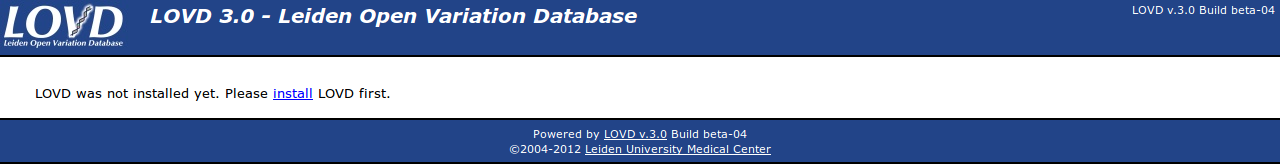
\includegraphics[width=\linewidth]{c02s02_screenshot_not_installed.png}%
  \caption{\footnotesize% % I want to format the captions better, but I'm having issues (see package loading comments).
    When pointing your browser to the LOVD location, it will tell you it's not installed yet.
    Click the link to start the install process.}
\end{figure}

LOVD will first check a few requirements.
Both the PHP and MySQL versions will be checked, to make sure your LOVD will function properly on your webserver environment.
Also some settings of the web server, PHP and MySQL will be checked.
Finally, LOVD will check if your config file has been hidden.
If all looks well, LOVD will tell you all requirements are OK and you're ready to start installing LOVD.
\\
\par
Installing LOVD consists of only 4 simple steps and will take only a couple of minutes, or less.

\begin{figure}[h]
  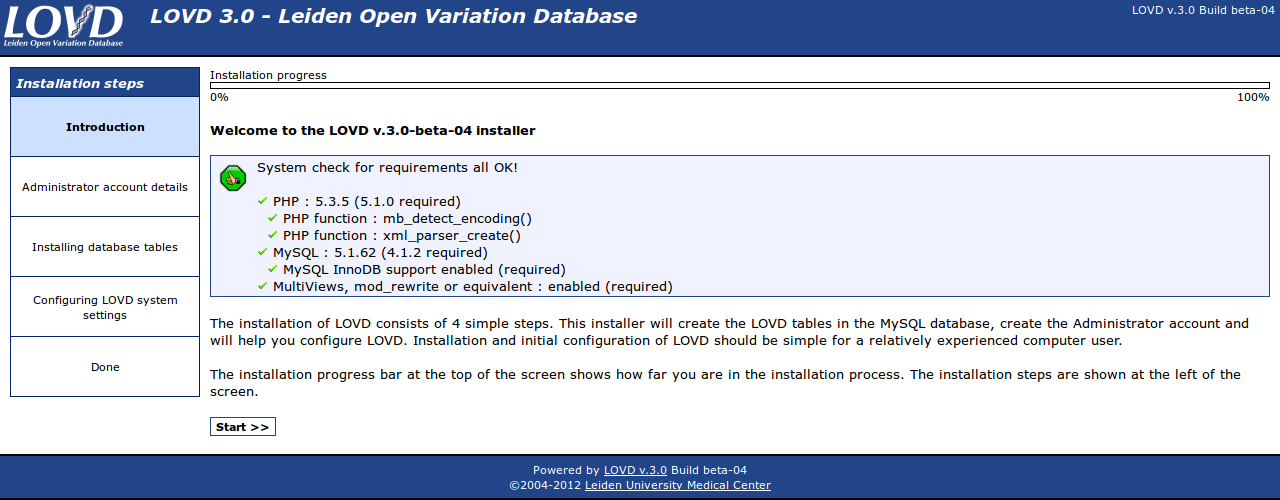
\includegraphics[width=\linewidth]{c02s02_screenshot_installer_01.png}%
  \caption{\footnotesize% % I want to format the captions better, but I'm having issues (see package loading comments).
    If all requirements are OK, you're ready to start installing LOVD.}
\end{figure}



\subsection{Administrator account details}
Fill in the database administrator data to install LOVD.
The database administrator will be the first user registered with LOVD and has full access to all of LOVD's functionalities.
The database administrator is the only user capable of creating manager accounts.
Managers can only create curator and submitter accounts.

\begin{figure}[h]
  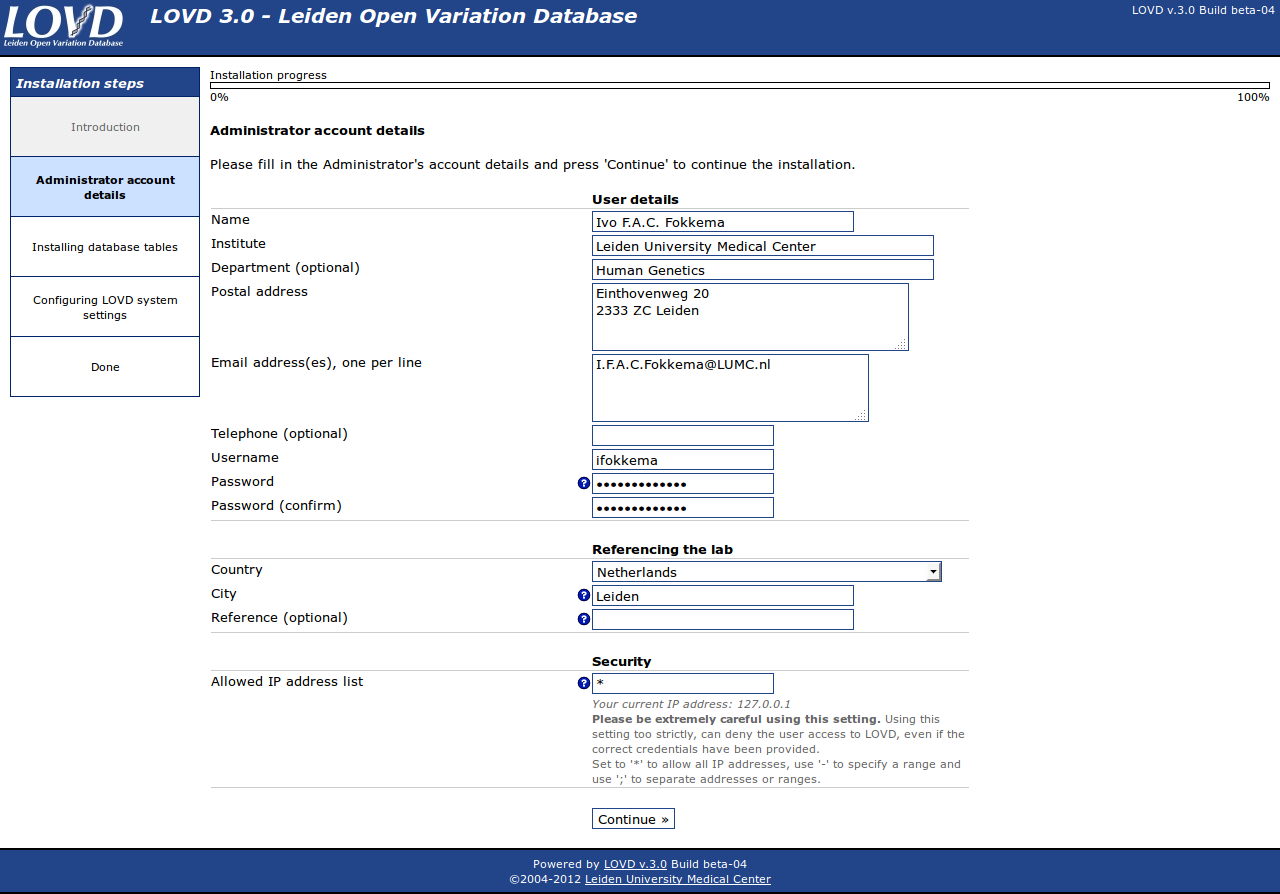
\includegraphics[width=\linewidth]{c02s02_screenshot_installer_02.png}%
  \caption{\footnotesize% % I want to format the captions better, but I'm having issues (see package loading comments).
    The database administrator registration form, with example data filled in.}
\end{figure}

Most of the form is pretty straight forward, but I will highlight one field - ``Allowed IP address list''.
An IP address is an address a computer is known by on the network.
To help prevent others to try and guess the username/password combination,
you can restrict access to the database administrator account to a number of IP addresses or ranges.
This also means you need to be very careful with this setting, as being too restrictive may lock you out of your account.
The default, unrestricted, value is *.

\begin{infotable}
The database administrator is the absolute owner of the LOVD installation.
Not only is he the only one that can uninstall LOVD from the database using the uninstaller,
he will also be able to create, edit or delete all user accounts in the system and
(depending on the settings) receive submission and registration notifications.
\end{infotable}

After completing the database administrator account details, click the ``Continue \guillemotright'' button at the bottom.
LOVD will apply a simple username and password quality check.
If LOVD tells you that the provided details are OK, click the ``Next \guillemotright'' button.



\subsection{Installing database tables}
The next step is to create and fill all necessary LOVD database tables.
LOVD will do this automatically, and you can watch the progress bar complete while the tables are created,
the country list filled, the database administrator account created, the custom columns preconfigured,
the standard columns enabled, and the custom links generated.
This may take a while on non-optimal conditions, so please be patient.
When everything is done, a ``Next \guillemotright'' button appears - click it to continue.

\begin{figure}[h]
  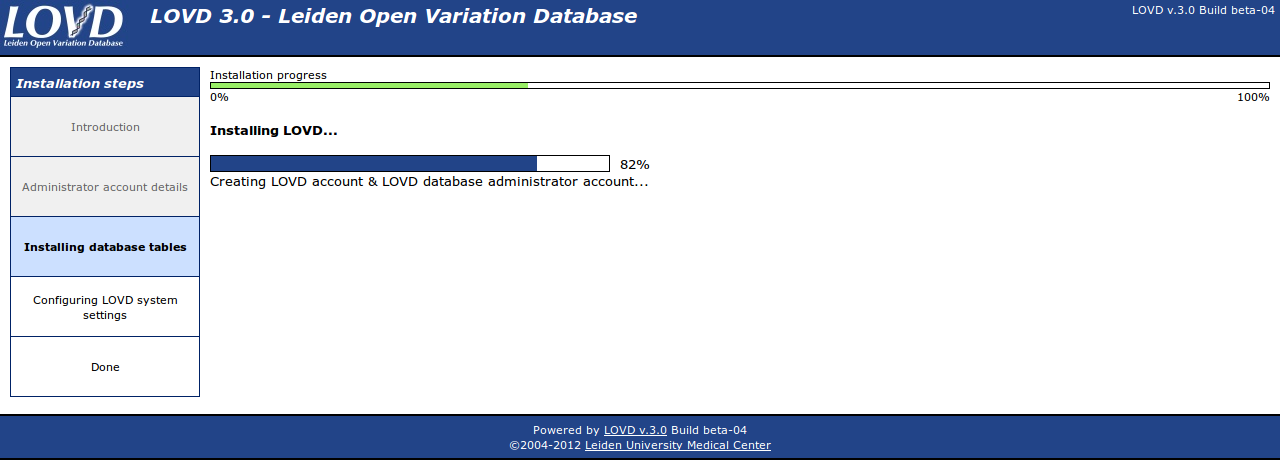
\includegraphics[width=\linewidth]{c02s02_screenshot_installer_03.png}%
  \caption{\footnotesize% % I want to format the captions better, but I'm having issues (see package loading comments).
    Watch the progress bar complete while LOVD informs you which part of the database table installation is currently in progress.}
\end{figure}



\subsection{Configuring LOVD system settings}
The final form in the installation process is completing the initial configuration of the LOVD system settings.
These settings can be changed after installation at any time through the LOVD setup.
\par
The only setting that cannot be changed at a later time, is the install lock, which is checked by default.
Setting the uninstall lock will prevent uninstallation of LOVD by the database administrator.
The only way to remove this lock is directly through the MySQL database backend.

\begin{figure}[h]
  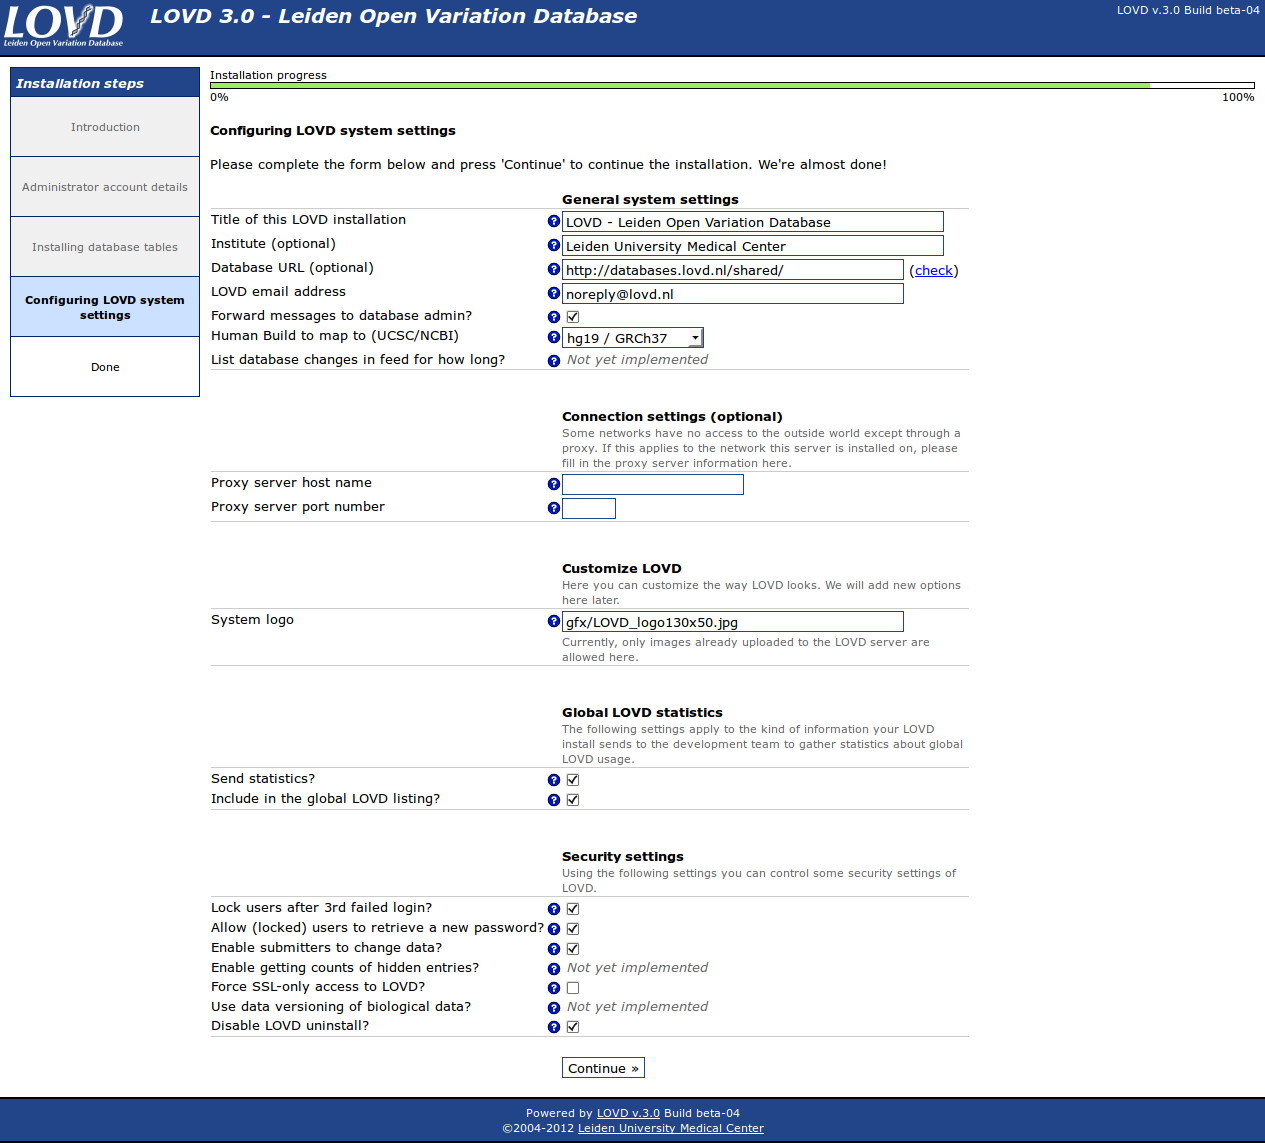
\includegraphics[width=\linewidth]{c02s02_screenshot_installer_04.png}%
  \caption{\footnotesize% % I want to format the captions better, but I'm having issues (see package loading comments).
    The system settings form, with example data filled in.}
\end{figure}

%For more information on the options of the LOVD system settings, see the LOVD system settings section of the manual.
%\\
%\par
After filling in the form, click ``Continue \guillemotright''.
If everything was filled in correctly, LOVD will register the LOVD system settings.
Click ``Next \guillemotright'' to continue to the last step.
Almost done!



\subsection{Done}
% FIXME; to be honest nothing is done in this step... so... kill it?
When everything has been filled in and stored correctly, the installation is complete.
Now that you're done installing LOVD, click the ``Continue to Setup area \guillemotright'' button to be forwarded to the LOVD setup area.
From there, you can perform the most important actions for managers in LOVD, such as creating new gene databases or disease information entries, registering new user accounts or authorizing curators, or manage the custom columns and links.
The button to create a new gene will be highlighted, as a suggestion of your next step!






%\chapter{Chapter...}



%\section{Section...}

%\subsection{Subsection...}

%\subsubsection{Subsubsection...}



%\begin{infobox}
%  \caption{\textbf{Caption}}
%  ...
%\end{infobox}






\end{document}





\chapter{}
\section{}
\subsection{}



$_PAGES =
     array(
            'LOVD Setup',
             array(
                    'LOVD system settings',
                    'Gene databases',
                     array(
                            'Creating new genes',
                            'Editing genes',
                            'Emptying genes',
                            'Deleting genes',
                          ),
                    'Custom columns',
                     array(
                            'Variant vs. patient columns',
                            'Managing patient columns',
                            'Creating new columns',
                            'Editing custom column default settings',
                            'Deleting custom columns',
                            'Downloading custom column data to text files',
                            'Importing custom columns from text files',
                          ),
                    'Authorized users',
                     array(
                            'Creating new users',
                            'Editing users',
                            'Locking users from the system',
                            'Deleting users',
                            'Assigning curators to specific genes',
                          ),
                    'Submitters',
                     array(
                            'Creating new submitters',
                            'Editing submitters',
                            'Deleting submitters',
                          ),
                    'Custom links',
                     array(
                            'Creating new links',
                            'Editing links',
                            'Deleting links',
                          ),
                    'Modules',
                     array(
                            'Installing modules',
                            'Enabling or disabling modules',
                            'Uninstalling modules',
                            'Available LOVD modules',
                          ),
                    'System logs',
                     array(
                            'What is logged by LOVD',
                            'Viewing and searching through the logs',
                            'Removing log entries',
                          ),
                    'Uninstalling LOVD',
                  ),
            'LOVD Gene configuration area',
             array(
                    'Gene settings',
                    'Custom variant columns',
                    'Curating variants',
                    'Download or import variants',
                    'Advanced edit features',
                     array(
                            'Find & Replace',
                            'Copy Column',
                          ),
                  ),
            'Gene homepage',
             array(
                    'News feed',
                  ),
            'Variant and patient data',
             array(
                    'Viewing and searching variant and patient data',
                     array(
                            'Advanced options',
                          ),
                    'Submitting variant and patient data',
                    'Editing variant data',
                    'Editing patient data',
                    'Deleting variant or patient data',
                    'Downloading data to text files',
                    'Importing text files',
                    'Database statistics',
                  ),
            'Submitters',
             array(
                    'Registering a new account',
                    'Keeping your account up to date',
                    'Keeping track of your submissions',
                  ),
            'LOVD scripts',
             array(
                    'Enabling the scripts',
                    'GenBank File Uploader',
                    'Reading Frame Checker',
                    'Reference Sequence Parser',
                  ),
            'Use of HTML within LOVD',
            'Updating LOVD',
            'Keeping your data secure',
          );




(couldn't get color into this one...)

\usepackage{fancybox} % New attempt for fancy boxes...

\newlength{\mylength}
\newenvironment{infotable}%
{\setlength{\fboxsep}{15pt}
\setlength{\mylength}{\linewidth}%
\addtolength{\mylength}{-2\fboxsep}%
\addtolength{\mylength}{-2\fboxrule}%
\addtolength{\mylength}{-1.5cm}%
\Sbox
\begin{minipage}[t]{1.5cm}

\includegraphics[width=1cm]{lovd_information.png}
\end{minipage}
\minipage{\mylength}%
}%
{\endminipage\endSbox
\[\fbox{\TheSbox}\]}


